\documentclass[14pt]{extbook}
\usepackage{multicol, enumerate, enumitem, hyperref, color, soul, setspace, parskip, fancyhdr} %General Packages
\usepackage{amssymb, amsthm, amsmath, latexsym, units, mathtools} %Math Packages
\everymath{\displaystyle} %All math in Display Style
% Packages with additional options
\usepackage[headsep=0.5cm,headheight=12pt, left=1 in,right= 1 in,top= 1 in,bottom= 1 in]{geometry}
\usepackage[usenames,dvipsnames]{xcolor}
\usepackage{dashrule}  % Package to use the command below to create lines between items
\newcommand{\litem}[1]{\item#1\hspace*{-1cm}\rule{\textwidth}{0.4pt}}
\pagestyle{fancy}
\lhead{Progress Quiz 7}
\chead{}
\rhead{Version A}
\lfoot{3510-5252}
\cfoot{}
\rfoot{Summer C 2021}
\begin{document}

\begin{enumerate}
\litem{
First, find the equation of the line containing the two points below. Then, write the equation in the form $ y=mx+b $ and choose the intervals that contain $m$ and $b$.\[ (6, -9) \text{ and } (4, 3) \]\begin{enumerate}[label=\Alph*.]
\item \( m \in [-6, -2] \hspace*{3mm} b \in [-16, -9] \)
\item \( m \in [-6, -2] \hspace*{3mm} b \in [-2, 1] \)
\item \( m \in [-6, -2] \hspace*{3mm} b \in [-29, -22] \)
\item \( m \in [-6, -2] \hspace*{3mm} b \in [24, 31] \)
\item \( m \in [2, 10] \hspace*{3mm} b \in [-25, -20] \)

\end{enumerate} }
\litem{
Write the equation of the line in the graph below in Standard Form $Ax+By=C$. Then, choose the intervals that contain $A, B, \text{ and } C$.
\begin{center}
    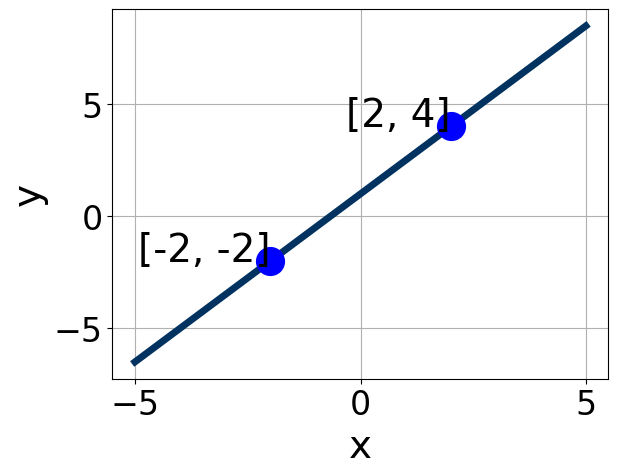
\includegraphics[width=0.5\textwidth]{../Figures/linearGraphToStandardCopyA.png}
\end{center}
\begin{enumerate}[label=\Alph*.]
\item \( A \in [2.84, 4.64], \hspace{3mm} B \in [-2.32, -1.44], \text{ and } \hspace{3mm} C \in [-2.02, -1.52] \)
\item \( A \in [-4.01, -2.79], \hspace{3mm} B \in [1.7, 2.01], \text{ and } \hspace{3mm} C \in [1.22, 3.88] \)
\item \( A \in [2.84, 4.64], \hspace{3mm} B \in [1.7, 2.01], \text{ and } \hspace{3mm} C \in [1.22, 3.88] \)
\item \( A \in [-2.92, -1.26], \hspace{3mm} B \in [0.95, 1.02], \text{ and } \hspace{3mm} C \in [0.78, 1.69] \)
\item \( A \in [-2.92, -1.26], \hspace{3mm} B \in [-1.83, -0.44], \text{ and } \hspace{3mm} C \in [-1.05, -0.64] \)

\end{enumerate} }
\litem{
Solve the equation below. Then, choose the interval that contains the solution.\[ -10(12x + 9) = -18(-19x + 17) \]\begin{enumerate}[label=\Alph*.]
\item \( x \in [-1.03, -0.42] \)
\item \( x \in [0.43, 0.78] \)
\item \( x \in [1.1, 2.23] \)
\item \( x \in [0.6, 1.61] \)
\item \( \text{There are no real solutions.} \)

\end{enumerate} }
\litem{
First, find the equation of the line containing the two points below. Then, write the equation in the form $ y=mx+b $ and choose the intervals that contain $m$ and $b$.\[ (11, -5) \text{ and } (-3, 11) \]\begin{enumerate}[label=\Alph*.]
\item \( m \in [0.14, 4.14] \hspace*{3mm} b \in [14.22, 14.87] \)
\item \( m \in [-3.14, 0.86] \hspace*{3mm} b \in [-16.3, -15.83] \)
\item \( m \in [-3.14, 0.86] \hspace*{3mm} b \in [13.94, 14.32] \)
\item \( m \in [-3.14, 0.86] \hspace*{3mm} b \in [-7.96, -7.54] \)
\item \( m \in [-3.14, 0.86] \hspace*{3mm} b \in [7.19, 8.06] \)

\end{enumerate} }
\litem{
Write the equation of the line in the graph below in Standard Form $Ax+By=C$. Then, choose the intervals that contain $A, B, \text{ and } C$.
\begin{center}
    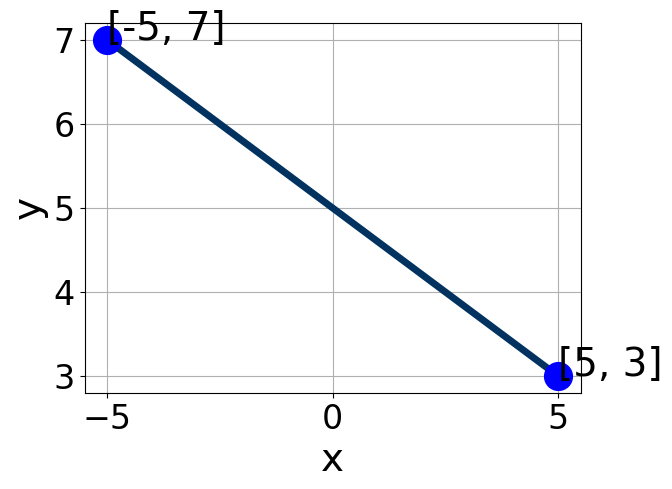
\includegraphics[width=0.5\textwidth]{../Figures/linearGraphToStandardA.png}
\end{center}
\begin{enumerate}[label=\Alph*.]
\item \( A \in [-1.7, 0.9], \hspace{3mm} B \in [-2.32, -0.17], \text{ and } \hspace{3mm} C \in [-7, -3] \)
\item \( A \in [1.6, 3.1], \hspace{3mm} B \in [-7.51, -4.95], \text{ and } \hspace{3mm} C \in [-29, -23] \)
\item \( A \in [-1.7, 0.9], \hspace{3mm} B \in [0.43, 2.07], \text{ and } \hspace{3mm} C \in [1, 12] \)
\item \( A \in [1.6, 3.1], \hspace{3mm} B \in [4.1, 5.67], \text{ and } \hspace{3mm} C \in [24, 31] \)
\item \( A \in [-2.6, 0.2], \hspace{3mm} B \in [-7.51, -4.95], \text{ and } \hspace{3mm} C \in [-29, -23] \)

\end{enumerate} }
\litem{
Solve the equation below. Then, choose the interval that contains the solution.\[ -12(11x -16) = -8(-14x -6) \]\begin{enumerate}[label=\Alph*.]
\item \( x \in [-0.09, 0.98] \)
\item \( x \in [0.87, 0.99] \)
\item \( x \in [11.94, 12.19] \)
\item \( x \in [-1.3, -0.55] \)
\item \( \text{There are no real solutions.} \)

\end{enumerate} }
\litem{
Solve the linear equation below. Then, choose the interval that contains the solution.\[ \frac{4x + 5}{5} - \frac{-3x -8}{2} = \frac{-7x + 3}{8} \]\begin{enumerate}[label=\Alph*.]
\item \( x \in [-0.38, 0.07] \)
\item \( x \in [-4.29, -2.18] \)
\item \( x \in [-2.82, -1.42] \)
\item \( x \in [0.98, 1.57] \)
\item \( \text{There are no real solutions.} \)

\end{enumerate} }
\litem{
Find the equation of the line described below. Write the linear equation in the form $ y=mx+b $ and choose the intervals that contain $m$ and $b$.\[ \text{Perpendicular to } 8 x - 9 y = 9 \text{ and passing through the point } (-9, 4). \]\begin{enumerate}[label=\Alph*.]
\item \( m \in [-1.33, -0.98] \hspace*{3mm} b \in [5.49, 6.27] \)
\item \( m \in [-0.99, -0.73] \hspace*{3mm} b \in [-6.39, -4.95] \)
\item \( m \in [-1.33, -0.98] \hspace*{3mm} b \in [12.5, 13.4] \)
\item \( m \in [0.85, 1.49] \hspace*{3mm} b \in [13.67, 14.79] \)
\item \( m \in [-1.33, -0.98] \hspace*{3mm} b \in [-6.39, -4.95] \)

\end{enumerate} }
\litem{
Solve the linear equation below. Then, choose the interval that contains the solution.\[ \frac{4x + 5}{7} - \frac{8x + 7}{5} = \frac{-3x + 6}{4} \]\begin{enumerate}[label=\Alph*.]
\item \( x \in [-3.19, -1.19] \)
\item \( x \in [1.21, 3.21] \)
\item \( x \in [-9.85, -4.85] \)
\item \( x \in [-30.72, -27.72] \)
\item \( \text{There are no real solutions.} \)

\end{enumerate} }
\litem{
Find the equation of the line described below. Write the linear equation in the form $ y=mx+b $ and choose the intervals that contain $m$ and $b$.\[ \text{Parallel to } 8 x - 9 y = 15 \text{ and passing through the point } (4, 9). \]\begin{enumerate}[label=\Alph*.]
\item \( m \in [0.72, 0.92] \hspace*{3mm} b \in [-8.4, -4] \)
\item \( m \in [1.09, 1.37] \hspace*{3mm} b \in [5.2, 5.7] \)
\item \( m \in [0.72, 0.92] \hspace*{3mm} b \in [5.2, 5.7] \)
\item \( m \in [-0.94, -0.66] \hspace*{3mm} b \in [11.2, 13.6] \)
\item \( m \in [0.72, 0.92] \hspace*{3mm} b \in [2.2, 5.3] \)

\end{enumerate} }
\end{enumerate}

\end{document}